\documentclass[11pt,a4paper]{article}
\newcommand{\intestazione}{Dimero di spin --- 2. VQE}
% =====================================================================
%  Preambolo comune ai documenti sul dimero (serie "che cosa abbiamo fatto")
%  Incluso con % =====================================================================
%  Preambolo comune ai documenti sul dimero (serie "che cosa abbiamo fatto")
%  Incluso con % =====================================================================
%  Preambolo comune ai documenti sul dimero (serie "che cosa abbiamo fatto")
%  Incluso con \input{preambolo_dimero} subito dopo \documentclass.
% =====================================================================
\usepackage[T1]{fontenc}
\usepackage[utf8]{inputenc}
\usepackage[main=italian,provide=*]{babel}
\usepackage{amsmath,amssymb,mathtools}
\usepackage{graphicx}
\usepackage{booktabs}
\usepackage{colortbl}
\usepackage{xcolor}
\usepackage{geometry}
\usepackage{placeins}
\usepackage{caption}
\usepackage{enumitem}
\usepackage{fancyhdr}
\usepackage{needspace}
\usepackage{tikz}
\usetikzlibrary{arrows.meta,positioning,shapes.geometric,calc,fit,backgrounds}
\usepackage{hyperref}
\hypersetup{colorlinks=true,linkcolor=blu,citecolor=blu,urlcolor=blu}

\geometry{margin=2.5cm}

% --- colori coerenti con quelli delle figure (palette Okabe-Ito)
\definecolor{blu}{HTML}{0072B2}
\definecolor{arancio}{HTML}{E69F00}
\definecolor{verdes}{HTML}{009E73}
\definecolor{rossos}{HTML}{D55E00}
\definecolor{violas}{HTML}{CC79A7}
\definecolor{grigetto}{HTML}{E8E8E8}

\captionsetup{font=small,labelfont=bf,width=0.92\textwidth}

\pagestyle{fancy}
\fancyhf{}
\fancyhead[L]{\small\itshape\intestazione}
\fancyhead[R]{\small\thepage}
\renewcommand{\headrulewidth}{0.3pt}

% --- notazione
\newcommand{\ket}[1]{\lvert #1\rangle}
\newcommand{\bra}[1]{\langle #1 \rvert}
\newcommand{\media}[1]{\langle #1 \rangle}
\newcommand{\vs}[1]{\mathbf{s}_{#1}}

% --- riquadro "in una riga": il messaggio da portare a casa
\newcommand{\messaggio}[1]{%
  \begin{center}
  \begin{minipage}{0.93\textwidth}
  \setlength{\fboxsep}{9pt}%
  \colorbox{grigetto}{\begin{minipage}{\dimexpr\textwidth-2\fboxsep}
  \small\textbf{In una riga.}\enspace #1
  \end{minipage}}
  \end{minipage}
  \end{center}
}

% --- riquadro "come lo sappiamo": la verifica numerica dietro un'affermazione
\newcommand{\verifica}[1]{%
  \begin{center}
  \begin{minipage}{0.93\textwidth}
  \small\textcolor{verdes}{\rule{2.2em}{1.1pt}}\enspace
  \textcolor{verdes}{\textbf{Come lo sappiamo.}}\enspace #1
  \end{minipage}
  \end{center}
  \medskip
}
 subito dopo \documentclass.
% =====================================================================
\usepackage[T1]{fontenc}
\usepackage[utf8]{inputenc}
\usepackage[main=italian,provide=*]{babel}
\usepackage{amsmath,amssymb,mathtools}
\usepackage{graphicx}
\usepackage{booktabs}
\usepackage{colortbl}
\usepackage{xcolor}
\usepackage{geometry}
\usepackage{placeins}
\usepackage{caption}
\usepackage{enumitem}
\usepackage{fancyhdr}
\usepackage{needspace}
\usepackage{tikz}
\usetikzlibrary{arrows.meta,positioning,shapes.geometric,calc,fit,backgrounds}
\usepackage{hyperref}
\hypersetup{colorlinks=true,linkcolor=blu,citecolor=blu,urlcolor=blu}

\geometry{margin=2.5cm}

% --- colori coerenti con quelli delle figure (palette Okabe-Ito)
\definecolor{blu}{HTML}{0072B2}
\definecolor{arancio}{HTML}{E69F00}
\definecolor{verdes}{HTML}{009E73}
\definecolor{rossos}{HTML}{D55E00}
\definecolor{violas}{HTML}{CC79A7}
\definecolor{grigetto}{HTML}{E8E8E8}

\captionsetup{font=small,labelfont=bf,width=0.92\textwidth}

\pagestyle{fancy}
\fancyhf{}
\fancyhead[L]{\small\itshape\intestazione}
\fancyhead[R]{\small\thepage}
\renewcommand{\headrulewidth}{0.3pt}

% --- notazione
\newcommand{\ket}[1]{\lvert #1\rangle}
\newcommand{\bra}[1]{\langle #1 \rvert}
\newcommand{\media}[1]{\langle #1 \rangle}
\newcommand{\vs}[1]{\mathbf{s}_{#1}}

% --- riquadro "in una riga": il messaggio da portare a casa
\newcommand{\messaggio}[1]{%
  \begin{center}
  \begin{minipage}{0.93\textwidth}
  \setlength{\fboxsep}{9pt}%
  \colorbox{grigetto}{\begin{minipage}{\dimexpr\textwidth-2\fboxsep}
  \small\textbf{In una riga.}\enspace #1
  \end{minipage}}
  \end{minipage}
  \end{center}
}

% --- riquadro "come lo sappiamo": la verifica numerica dietro un'affermazione
\newcommand{\verifica}[1]{%
  \begin{center}
  \begin{minipage}{0.93\textwidth}
  \small\textcolor{verdes}{\rule{2.2em}{1.1pt}}\enspace
  \textcolor{verdes}{\textbf{Come lo sappiamo.}}\enspace #1
  \end{minipage}
  \end{center}
  \medskip
}
 subito dopo \documentclass.
% =====================================================================
\usepackage[T1]{fontenc}
\usepackage[utf8]{inputenc}
\usepackage[main=italian,provide=*]{babel}
\usepackage{amsmath,amssymb,mathtools}
\usepackage{graphicx}
\usepackage{booktabs}
\usepackage{colortbl}
\usepackage{xcolor}
\usepackage{geometry}
\usepackage{placeins}
\usepackage{caption}
\usepackage{enumitem}
\usepackage{fancyhdr}
\usepackage{needspace}
\usepackage{tikz}
\usetikzlibrary{arrows.meta,positioning,shapes.geometric,calc,fit,backgrounds}
\usepackage{hyperref}
\hypersetup{colorlinks=true,linkcolor=blu,citecolor=blu,urlcolor=blu}

\geometry{margin=2.5cm}

% --- colori coerenti con quelli delle figure (palette Okabe-Ito)
\definecolor{blu}{HTML}{0072B2}
\definecolor{arancio}{HTML}{E69F00}
\definecolor{verdes}{HTML}{009E73}
\definecolor{rossos}{HTML}{D55E00}
\definecolor{violas}{HTML}{CC79A7}
\definecolor{grigetto}{HTML}{E8E8E8}

\captionsetup{font=small,labelfont=bf,width=0.92\textwidth}

\pagestyle{fancy}
\fancyhf{}
\fancyhead[L]{\small\itshape\intestazione}
\fancyhead[R]{\small\thepage}
\renewcommand{\headrulewidth}{0.3pt}

% --- notazione
\newcommand{\ket}[1]{\lvert #1\rangle}
\newcommand{\bra}[1]{\langle #1 \rvert}
\newcommand{\media}[1]{\langle #1 \rangle}
\newcommand{\vs}[1]{\mathbf{s}_{#1}}

% --- riquadro "in una riga": il messaggio da portare a casa
\newcommand{\messaggio}[1]{%
  \begin{center}
  \begin{minipage}{0.93\textwidth}
  \setlength{\fboxsep}{9pt}%
  \colorbox{grigetto}{\begin{minipage}{\dimexpr\textwidth-2\fboxsep}
  \small\textbf{In una riga.}\enspace #1
  \end{minipage}}
  \end{minipage}
  \end{center}
}

% --- riquadro "come lo sappiamo": la verifica numerica dietro un'affermazione
\newcommand{\verifica}[1]{%
  \begin{center}
  \begin{minipage}{0.93\textwidth}
  \small\textcolor{verdes}{\rule{2.2em}{1.1pt}}\enspace
  \textcolor{verdes}{\textbf{Come lo sappiamo.}}\enspace #1
  \end{minipage}
  \end{center}
  \medskip
}


\title{\bfseries Trovare lo stato fondamentale con un circuito\\[2pt]
\large Documento 2 --- VQE, e perché la scelta dell'ansatz è il vero risultato}
\author{Samuele Schiavi \\ \small Tesi triennale in Fisica, Università di Parma
--- Relatore: Prof.\ Alessandro Chiesa}
\date{}

\begin{document}
\maketitle
\thispagestyle{fancy}

\section{Come funziona, in pratica}

Il Variational Quantum Eigensolver risolve un problema di minimo. Si costruisce
un circuito quantistico che dipende da un insieme di angoli
$\boldsymbol\theta$; il circuito prepara uno stato
$\ket{\psi(\boldsymbol\theta)}$; si misura l'energia media
$E(\boldsymbol\theta)=\bra{\psi(\boldsymbol\theta)}H\ket{\psi(\boldsymbol\theta)}$;
un ottimizzatore classico aggiorna gli angoli per abbassarla. Il principio
variazionale garantisce che $E(\boldsymbol\theta)\ge E_0$ sempre: non si può
scendere sotto il valore vero.

\begin{figure}[htbp]
\centering
\begin{tikzpicture}[
  q/.style={draw,rounded corners=3pt,fill=blu!8,draw=blu,thick,
            minimum height=1.3cm,minimum width=3.5cm,align=center,font=\small},
  c/.style={draw,rounded corners=3pt,fill=arancio!12,draw=arancio,thick,
            minimum height=1.3cm,minimum width=3.5cm,align=center,font=\small},
  fr/.style={-{Stealth[length=2.6mm]},thick,gray}]
\node[q] (prep) at (0,0)   {circuito parametrico\\ $\ket{\psi(\boldsymbol\theta)}$};
\node[q] (mis)  at (5,0)   {misura di\\ $\media{H}$};
\node[c] (opt)  at (10,0)  {ottimizzatore\\ classico};
\draw[fr] (prep) -- (mis);
\draw[fr] (mis)  -- (opt);
\draw[fr] (opt.south) -- ++(0,-1.05) -- node[below,font=\scriptsize,text=black]
   {nuovi angoli $\boldsymbol\theta$} ++(-10,0) -- (prep.south);
\node[font=\scriptsize,text=gray] at (2.5,0.95) {parte quantistica};
\node[font=\scriptsize,text=gray] at (10,0.95) {parte classica};
\end{tikzpicture}
\caption{Il ciclo VQE. La macchina quantistica prepara e misura; l'ottimizzatore
classico decide dove muoversi. L'unica cosa che il fisico sceglie è la struttura
del circuito parametrico --- ed è quella scelta a decidere se il metodo funziona.}
\end{figure}

\FloatBarrier

Sul dimero l'energia esatta è nota, quindi il VQE non serve a scoprirla: serve a
misurare quanto bene un dato circuito riesce a rappresentare lo stato giusto.
La grandezza che useremo è la \emph{fidelity}
$\mathcal F = \lvert\langle\psi_{\rm VQE}|\psi_0\rangle\rvert$, che vale $1$ quando i
due stati coincidono.

\medskip
\noindent\textbf{Esatto.} $\ket{\psi_0}$, lo stato fondamentale vero, da
diagonalizzazione diretta di $H$ (\texttt{np.linalg.eigh}) --- nessuna
approssimazione.

\noindent\textbf{Vero.} $\ket{\psi_{\rm VQE}}=\ket{\psi(\boldsymbol\theta^*)}$,
lo stato prodotto dal circuito ansatz con i parametri ottimali trovati dal
VQE --- genuinamente eseguito (\texttt{Statevector} sul circuito con i
parametri assegnati), mai una scorciatoia. Non c'è qui un terzo metodo da
confrontare, a differenza dei Documenti 3 e 4: ogni fidelity in questo
documento è già, sempre, un confronto diretto fra questi due.

\messaggio{Sul dimero il VQE è uno strumento diagnostico: mette alla prova
l'ansatz, non l'Hamiltoniana.}

\section{Due filosofie di circuito}

\subsection*{Ansatz generico (hardware-efficient)}

Si impilano rotazioni a un qubit e porte di entanglement in uno schema regolare,
senza guardare alla fisica del problema. Nel nostro caso: rotazioni $R_y$
alternate a porte $CZ$, per un totale di $6$ parametri.

\begin{figure}[htbp]
\centering

\includegraphics[width=0.62\textwidth]{figure/circ_ha}
\caption{L'ansatz generico. Nessuna informazione sul sistema è entrata nella sua
costruzione: la stessa struttura si userebbe per qualunque Hamiltoniana a due
qubit.}
\end{figure}

\FloatBarrier

\subsection*{Ansatz fisicamente motivato}

L'alternativa è costruire il circuito \emph{a partire} da quel che si sa dello
stato cercato. Sotto l'incrocio lo stato fondamentale è il singoletto, sopra è
$\ket{\!\downarrow\downarrow}$: si prepara direttamente lo stato giusto e si
aggiunge un blocco a due qubit con un angolo libero, che permette di
deformarlo. Un parametro invece di sei --- da qui in avanti lo chiamiamo
\textbf{ansatz base} (o \textbf{PMA base}): è l'ansatz con il minor numero
di parametri, ma ``base'' evita l'ambiguità con ``minimizzare l'energia'', che
è il verbo del VQE stesso, non un aggettivo per questo circuito.

Quel blocco è realizzato con due CNOT che racchiudono una rotazione
$R_y(\theta)$ su un solo qubit:

\begin{figure}[htbp]
\centering

\includegraphics[width=0.42\textwidth]{figure/circ_cnotry}
\caption{Il blocco a un parametro usato nell'ansatz base: due CNOT, non due
CZ, attorno a un'unica $R_y$. È una rotazione reale, confinata al
sottospazio a due dimensioni \emph{che contiene} lo stato di preparazione ---
$\{\ket{01},\ket{10}\}$ sotto l'incrocio (dove vive il singoletto, non da
solo ma insieme al tripletto $M=0$), $\{\ket{00},\ket{11}\}$ sopra (dove
$\ket{\!\downarrow\downarrow}=\ket{11}$ è uno dei due vettori di base, non
l'intero sottospazio).}
\label{fig:cnotry}
\end{figure}

Il circuito completo ha due forme, non una --- \textbf{un ramo diverso a
seconda di $b/J$}, scelto dalla stessa condizione che separa i due tratti
dello spettro in Fig.~\ref{fig:confronto}. È essenziale vederli entrambi,
non solo il primo, perché il blocco di Fig.~\ref{fig:cnotry} non può mai
lasciare il sottospazio in cui parte (lo vedremo tra poco): la scelta del
ramo giusto non è un dettaglio, è ciò che permette al circuito di
funzionare.

\begin{figure}[htbp]
\centering
\begin{minipage}{0.48\textwidth}
\centering

\includegraphics[width=0.92\textwidth]{figure/circ_pma_base}
\vspace{2pt}
\textbf{Ramo $b/J<2$}
\end{minipage}
\hfill
\begin{minipage}{0.48\textwidth}
\centering

\includegraphics[width=0.92\textwidth]{figure/circ_pma_base_ramo2}
\vspace{2pt}
\textbf{Ramo $b/J\geq2$}
\end{minipage}
\caption{L'ansatz fisicamente motivato nella sua forma minima, nei suoi due
rami. \textbf{A sinistra}, $b/J<2$: preparazione esplicita del singoletto
(le prime quattro porte: $X,H,\text{CNOT},X$) seguita dal blocco di
Fig.~\ref{fig:cnotry}. \textbf{A destra}, $b/J\geq2$: preparazione di
$\ket{\!\downarrow\downarrow}=\ket{11}$ (due porte $X$, una per qubit) seguita
dallo stesso identico blocco parametrizzato. Il circuito incorpora ciò che
sappiamo del problema --- quale dei due stati sia il fondamentale a $D=0$
in quel tratto --- invece di lasciarlo scoprire all'ottimizzatore.}
\label{fig:pma-base-due-rami}
\end{figure}

\FloatBarrier

\needspace{9\baselineskip}
\section{Il confronto, e dove si rompe}

\begin{figure}[htbp]
\centering
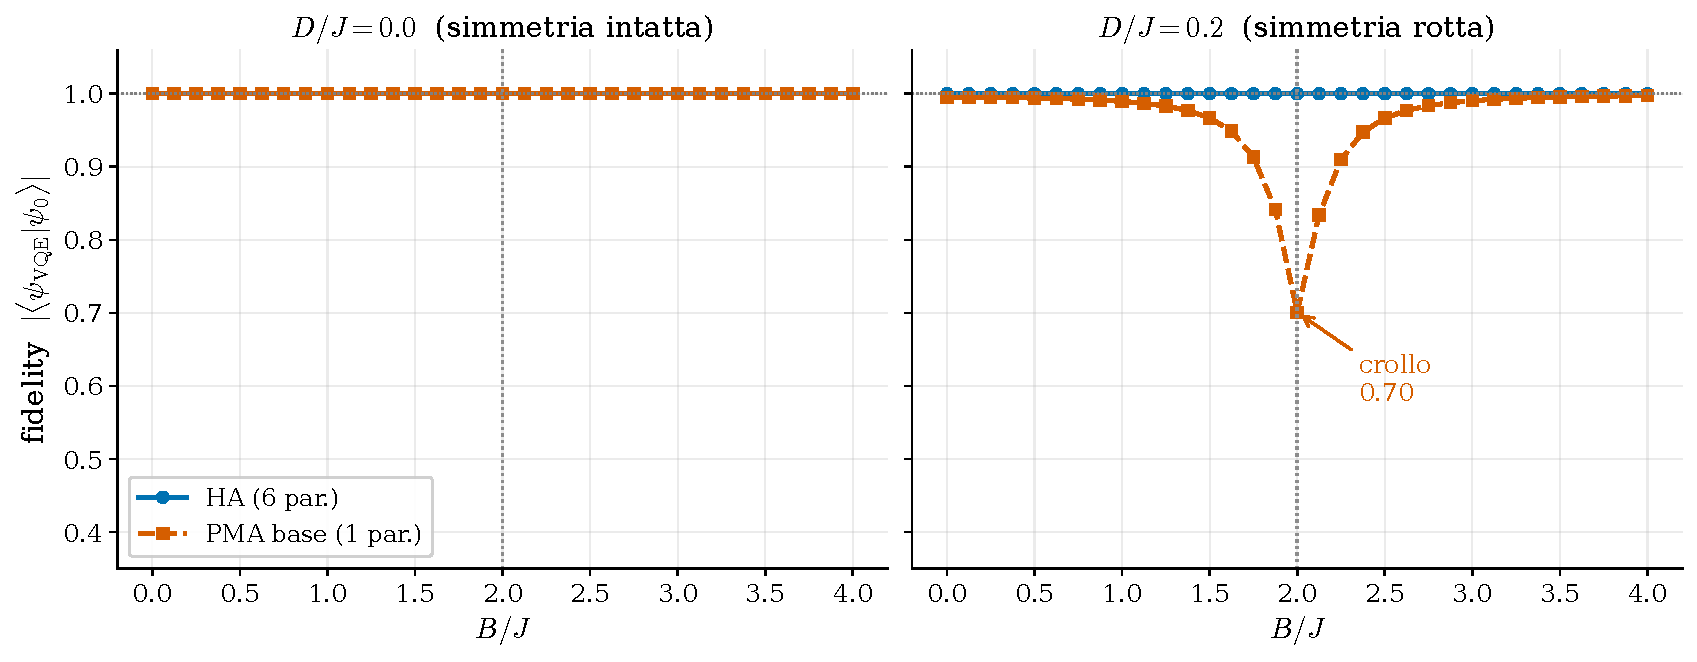
\includegraphics[width=\textwidth]{figure/fig03_vqe_ha_vs_pma}
\caption{Fidelity rispetto allo stato fondamentale esatto, al variare del campo.
\textbf{A sinistra}, senza termine DM: entrambi gli ansatz sono perfetti su
tutto il range, e quello a un parametro fa lo stesso lavoro di quello a sei.
\textbf{A destra}, con il DM acceso: l'ansatz generico resta perfetto, quello
fisicamente motivato crolla a $0.70$ proprio dove il DM conta di più.}
\label{fig:confronto}
\end{figure}

\FloatBarrier

Il pannello di sinistra è il risultato ``positivo'': imporre la simmetria giusta
riduce il costo di un fattore sei senza perdere nulla. È il messaggio centrale
di Crippa et al.\ (\emph{Magnetochemistry} \textbf{7}, 117, 2021), il
riferimento metodologico del progetto.

Il pannello di destra è il risultato più istruttivo. L'ansatz fisicamente
motivato fallisce, e fallisce in modo localizzato: lontano dall'incrocio va
benissimo, nell'intorno di $B/J=2$ perde un terzo della fidelity. La ragione
non è che ha pochi parametri.

Un dettaglio che vale la pena rendere esplicito, perché a un primo sguardo il
grafico sembra dire qualcosa di più forte di quello che dice davvero: il
circuito non prepara \emph{sempre} il singoletto. È costruito con due rami,
scelti a seconda di $B/J$: sotto l'incrocio prepara il singoletto, sopra
prepara $\ket{\!\downarrow\downarrow}=\ket{11}$.

Vale la pena essere precisi su \emph{dove} vivono questi due stati, perché
``vive nel sottospazio'' può suggerire più di quanto sia vero. Il singoletto
non occupa l'intero sottospazio a due dimensioni $\{\ket{01},\ket{10}\}$: è
una singola retta al suo interno,
$\ket{\psi^-}=\tfrac{1}{\sqrt2}(\ket{01}-\ket{10})$ --- una sola direzione,
non l'intero piano. Quello stesso sottospazio a due dimensioni contiene
anche il tripletto $M=0$,
$\ket{\Psi^+}=\tfrac{1}{\sqrt2}(\ket{01}+\ket{10})$: stessa ``casa'', ma
simmetria opposta (antisimmetrico il primo, simmetrico il secondo). In modo
speculare, $\ket{11}$ non è ``il sottospazio $\{\ket{00},\ket{11}\}$'': è
uno dei due vettori di base che lo generano --- l'altro, $\ket{00}$, è il
terzo stato di tripletto ($M=+1$), non uno stato qualsiasi. Il circuito, in
entrambi i rami, prepara sempre una singola retta precisa, mai l'intero
sottospazio a due dimensioni che la contiene.

Per chiarezza, la mappa completa dei quattro stati di spin totale rispetto
al registro di due qubit --- utile qui e ovunque nel seguito si parli di
settori a $M$ fissato:

\begin{table}[htbp]
\centering
\small
\renewcommand{\arraystretch}{1.3}
\begin{tabular}{@{}llll@{}}
\toprule
\rowcolor{grigetto}
\textbf{stato $\ket{S,M}$} & \textbf{stato di registro} & \textbf{settore ($M$)} & \textbf{tipo} \\
\midrule
$\ket{1,1}$ (tripletto) & $\ket{00}$ & $M=+1$, da solo & separabile \\
$\ket{1,0}$ (tripletto) & $\tfrac{1}{\sqrt2}(\ket{01}+\ket{10})$ & $M=0$, con il singoletto & entangled \\
$\ket{0,0}$ (singoletto) & $\tfrac{1}{\sqrt2}(\ket{01}-\ket{10})$ & $M=0$, con $\ket{1,0}$ & entangled \\
$\ket{1,-1}$ (tripletto) & $\ket{11}$ & $M=-1$, da solo & separabile \\
\bottomrule
\end{tabular}
\caption{I quattro stati di spin totale, verificato per ciascuno se sia
separabile (fattorizzabile come prodotto di due stati a un qubit,
verificato via SVD sulla matrice $2\times2$ delle ampiezze) o entangled. I
due settori $M=\pm1$ contengono un solo stato ciascuno --- $\ket{00}$ e
$\ket{11}$ non ``vivono in'' un sottospazio più grande, sono l'intero
settore, da soli. Il settore $M=0$ ne contiene invece due, e nessuno dei
due è separabile: sia il singoletto sia il tripletto $\ket{1,0}$ sono
combinazioni genuine di $\ket{01}$ e $\ket{10}$, non uno stato prodotto
scritto in modo complicato.}
\label{tab:quattro-stati-bell}
\end{table}

Il blocco a un parametro
ruota \emph{dentro} qualunque sottospazio sia partito, e non ne esce mai --- lo
si verifica applicandolo a entrambe le preparazioni per diversi valori
dell'angolo: le ampiezze restano rigorosamente nulle sulle due componenti non
raggiungibili da quel ramo, per ogni $\theta$.

\begin{figure}[htbp]
\centering
\begin{tikzpicture}[
  box/.style={draw,rounded corners=3pt,thick,align=center,font=\small,
              minimum width=4.5cm,minimum height=2.7cm,inner sep=6pt},
  lab/.style={font=\scriptsize,text=gray}]
\node[box,draw=blu,fill=blu!6] (L) at (0,0)
  {$B/J<2$: prepara $\ket{\text{singoletto}}$\\[3pt]
   $\downarrow$ CNOT--$R_y(\theta)$--CNOT\\[3pt]
   resta in $\{\ket{01},\ket{10}\}$ per ogni $\theta$};
\node[box,draw=arancio,fill=arancio!10] (R) at (6.0,0)
  {$B/J\ge2$: prepara $\ket{\!\downarrow\downarrow}$\\[3pt]
   $\downarrow$ CNOT--$R_y(\theta)$--CNOT\\[3pt]
   resta in $\{\ket{00},\ket{11}\}$ per ogni $\theta$};
\draw[dashed,thick,gray] (3.0,-1.7) -- (3.0,1.7);
\node[lab] at (3.0,1.95) {confine $B/J=2$};
\node[lab,text width=7.2cm,align=center] at (3.0,-2.15)
  {i due sottospazi non si toccano mai: nessun $\theta$, in nessuno dei due
   rami, produce ampiezza nell'altro};
\end{tikzpicture}
\caption{I due rami del circuito minimo, visti come due sottospazi disgiunti.
Il singolo parametro $\theta$ ruota liberamente \emph{dentro} il sottospazio a
due dimensioni di partenza, ma non può mai farlo uscire verso l'altro: sono
due piani distinti dentro lo spazio a quattro dimensioni, che si incontrano
solo nell'origine --- non un unico spazio esplorato per intero.}
\label{fig:due-rami}
\end{figure}

\FloatBarrier

Quindi per $B/J>2$ il circuito non sta più cercando (male) il singoletto: è
nel settore giusto per costruzione. Ma «giusto» non vuol dire «esatto». Il
termine DM accoppia $\ket{00}$ e $\ket{11}$ direttamente al settore
$\{\ket{01},\ket{10}\}$ (gli elementi di matrice di $X_1Z_2$ e $Z_1X_2$ lo
mostrano esplicitamente), quindi il vero stato fondamentale porta sempre un po'
di quel settore con sé, anche lontano dall'incrocio --- solo, sempre meno
quanto più ci si allontana:

\begin{table}[htbp]
\centering
\small
\renewcommand{\arraystretch}{1.25}
\begin{tabular}{@{}rcc@{}}
\toprule
\rowcolor{grigetto}
$B/J$ & fidelity & $1-\mathcal F$ \\
\midrule
0.00 & 0.995133 & $4.9\times10^{-3}$ \\
1.80 & 0.890358 & $1.1\times10^{-1}$ \\
1.99 & 0.725176 & $2.7\times10^{-1}$ \\
\textbf{2.00} & \textbf{0.700841} & $3.0\times10^{-1}$ \\
2.05 & 0.760745 & $2.4\times10^{-1}$ \\
2.50 & 0.966592 & $3.3\times10^{-2}$ \\
4.00 & 0.997527 & $2.5\times10^{-3}$ \\
\bottomrule
\end{tabular}
\caption{La fidelity dell'ansatz base, punto per punto. Lontano
dall'incrocio è un'ottima approssimazione ($\mathcal F>0.99$), non una
corrispondenza esatta: sulla scala del grafico di Fig.~\ref{fig:confronto}
(che parte da $0.4$) uno scarto dello $0.5\%$ è semplicemente invisibile, e la
curva sembra ``tornare a 1'' dove in realtà si avvicina soltanto. La stessa
fisica del Documento 1 vista da un altro angolo: la mescolanza indotta dal DM è
enorme esattamente dove i livelli imperturbati sono degeneri, e si affievolisce
rapidamente allontanandosene.}
\label{tab:fidelity-branch}
\end{table}

\FloatBarrier

Una domanda naturale a questo punto: la scelta del ramo (la condizione
$B/J<2$) è sempre quella giusta, cioè sceglie sempre il ramo che darebbe la
fidelity migliore? Quasi sempre --- ma non proprio esattamente:

\begin{table}[htbp]
\centering
\small
\renewcommand{\arraystretch}{1.25}
\begin{tabular}{@{}rccl@{}}
\toprule
\rowcolor{grigetto}
$B/J$ & fid(singoletto) & fid($\ket{\downarrow\downarrow}$) & ramo scelto dal codice \\
\midrule
1.90 & 0.8206 & 0.5707 & singoletto (il migliore) \\
1.99 & 0.7252 & 0.6881 & singoletto (il migliore) \\
\textbf{2.00} & \textbf{0.7129} & \textbf{0.7008} & $\ket{\downarrow\downarrow}$ --- \textbf{non} il migliore \\
2.01 & 0.7004 & 0.7134 & $\ket{\downarrow\downarrow}$ (il migliore) \\
2.10 & 0.5832 & 0.8121 & $\ket{\downarrow\downarrow}$ (il migliore) \\
\bottomrule
\end{tabular}
\caption{Cosa darebbe \emph{ciascun} ramo se venisse forzato su tutto il
range, confrontato con quale ramo la condizione $B/J<2$ sceglie davvero. La
scelta coincide quasi sempre con la migliore possibile fra le due --- tranne
esattamente al confine, $B/J=2$, dove per un margine sottile sceglie quella
peggiore ($0.7008$ invece di $0.7129$): un artefatto dello spigolo del
confronto ``$<$'', non un errore concettuale. Il minimo mostrato in
Fig.~\ref{fig:confronto} è dunque quello davvero prodotto dal codice, non il
minimo teoricamente raggiungibile da un selettore di ramo ottimale.}
\label{tab:doppio-ramo}
\end{table}

\FloatBarrier

Il punto di fondo non cambia: nessuno dei due rami esplora mai l'altro
\emph{simultaneamente} (Fig.~\ref{fig:due-rami}) --- il circuito non calcola
mai una sovrapposizione dei due, sceglie classicamente uno dei due prima
ancora di girare l'unico angolo che possiede. È precisamente perché un solo
parametro reale non può fare di meglio che serve una struttura diversa: la
riparazione di Sez.~\ref{sec:riparazione}, che segue, non aggiunge un secondo
ramo più furbo --- elimina la necessità di sceglierne uno.

\needspace{9\baselineskip}
\section{Perché non è una questione di parametri}

Con il DM acceso, lo stato fondamentale vicino all'incrocio è una miscela
\begin{equation}
\ket{\psi_0} = \alpha\ket{\text{singoletto}} + \beta\ket{\!\downarrow\downarrow},
\end{equation}
cioè una sovrapposizione di due stati con magnetizzazione diversa. L'ansatz
fisicamente motivato, costruito con blocchi che conservano $M$, resta confinato
in un settore: quello stato è fuori dalla sua portata, letteralmente
irraggiungibile.

Il modo per dimostrarlo senza margine di dubbio è aggiungere parametri e vedere
che non serve a nulla: ripetiamo $K$ volte il blocco CNOT--$R_y$--CNOT di
Fig.~\ref{fig:cnotry} (lo stesso già introdotto, non un gate nuovo), ciascuna
copia con il proprio angolo indipendente, a partire dallo stesso ramo che il
circuito sceglie a $B/J=2$ (il ramo $\ket{\!\downarrow\downarrow}$: la
condizione ``$B/J<2$'' è falsa esattamente nel punto di confine).

\begin{table}[htbp]
\centering
\small
\renewcommand{\arraystretch}{1.3}
\begin{tabular}{@{}ccc@{}}
\toprule
\rowcolor{grigetto}
\textbf{blocchi CNOT--$R_y$--CNOT} & \textbf{parametri} & \textbf{fidelity a $B/J=2$, $D/J=0.2$} \\
\midrule
1 & 1 & $0.700841$ \\
2 & 2 & $0.700841$ \\
3 & 3 & $0.700841$ \\
4 & 4 & $0.700841$ \\
\bottomrule
\end{tabular}
\caption{Il tetto strutturale. Quadruplicare i parametri non sposta la fidelity
di una sola cifra decimale --- e il valore coincide esattamente con quello di
un solo blocco (il minimo di Fig.~\ref{fig:confronto}): l'ottimizzatore sta già
facendo il meglio possibile dentro il settore in cui è confinato. Il limite non
è la capacità espressiva del circuito, è la simmetria che gli abbiamo imposto.
Ripetere lo stesso blocco confinato allo stesso sottospazio non aggiunge
direzioni raggiungibili, qualunque sia $K$.}
\label{tab:tetto}
\end{table}

\FloatBarrier

\messaggio{Un ansatz che rispetta una simmetria dell'Hamiltoniana è enormemente
più efficiente. Un ansatz che rispetta una simmetria che l'Hamiltoniana
\emph{non} ha è strutturalmente incapace, e nessun numero di parametri lo
salva.}

\needspace{9\baselineskip}
\section{La riparazione}
\label{sec:riparazione}
\label{sec:rbs-vs-w}

Prima di mostrare la cura, una parentesi necessaria: il blocco $M$-conservante
che useremo da qui in avanti non è quello di Fig.~\ref{fig:cnotry}, ma un altro,
diverso --- RBS. Vale la pena costruirlo con cura, vederne la matrice, e solo
alla fine confrontarlo con l'alternativa di letteratura.

\subsection*{RBS: una rotazione di Givens}

Applicando RBS$(\varphi)$ ai quattro stati della base computazionale si ottiene,
per verifica diretta:
\begin{equation}
\mathrm{RBS}(\varphi) =
\begin{pmatrix}
1 & 0 & 0 & 0\\
0 & \cos\varphi & -\sin\varphi & 0\\
0 & \sin\varphi & \cos\varphi & 0\\
0 & 0 & 0 & 1
\end{pmatrix}, \qquad \text{base } \{\ket{00},\ket{01},\ket{10},\ket{11}\}.
\end{equation}
Una matrice interamente \emph{reale}, identità su $\ket{00}$ e $\ket{11}$, e una
rotazione ordinaria $2\times2$ sul piano $\{\ket{01},\ket{10}\}$. Questa è
esattamente, per definizione, una \textbf{rotazione di Givens}: un operatore
ortogonale che ruota un solo piano coordinato di uno spazio più grande,
lasciando invariato tutto il resto. Non è un'analogia --- è il nome proprio
dell'oggetto.

La ragione per cui basta una rotazione di Givens, e non serve esplorare
l'intero gruppo unitario $U(2)$ del settore $M=0$, è il \textbf{teorema
spettrale}: una matrice reale simmetrica come la nostra $H$ ammette sempre una
base di autovettori reali, qualunque sia la degenerazione. Lo stato
fondamentale che l'ansatz deve raggiungere è reale; un operatore che deve
portare uno stato reale in un altro stato reale, restando dentro un piano a
due dimensioni, non ha bisogno di fasi complesse --- gli basta ruotare, cioè
gli basta essere una rotazione di Givens. RBS lo è per costruzione.

\begin{figure}[htbp]
\centering

\includegraphics[width=0.72\textwidth]{figure/circ_rbs_espanso}
\caption{RBS$(\varphi)$ nelle sue porte elementari: due CZ attorno a una
coppia di rotazioni $R_y(\varphi),R_y(-\varphi)$, sandwiched fra Hadamard. Due
porte a due qubit in tutto.}
\label{fig:rbs-espanso}
\end{figure}

\FloatBarrier

\subsection*{L'alternativa di letteratura: $W_{ij}(\theta)$}

In letteratura (Crippa et al.) il blocco $M$-conservante standard non è RBS: è
\begin{equation}
W_{ij}(\theta) = e^{-i\theta\,\vs i\cdot\vs j}, \qquad \vs{} = \boldsymbol\sigma/2.
\end{equation}
Nella stessa base:
\begin{equation}
W_{ij}(\theta) = e^{i\theta/4}
\begin{pmatrix}
e^{-i\theta/2} & 0 & 0 & 0\\
0 & \cos(\theta/2) & -i\sin(\theta/2) & 0\\
0 & -i\sin(\theta/2) & \cos(\theta/2) & 0\\
0 & 0 & 0 & e^{-i\theta/2}
\end{pmatrix}.
\end{equation}
A meno della fase globale davanti, il blocco $2\times2$ centrale ha la stessa
struttura $\cos,\sin$ di RBS ma con un fattore $-i$ davanti al seno: non è una
rotazione reale, è nella famiglia iSWAP. $\vs i\cdot\vs j$ è diagonale nella
base singoletto/tripletto, con autovalori $\tfrac14$ (tripletto) e
$-\tfrac34$ (singoletto) --- una fase relativa fra i due settori, non una
rotazione.

$W_{ij}(\theta)$ ha anch'esso una realizzazione esatta in porte elementari:
scrivendo $\vs i\cdot\vs j=\tfrac14(X_iX_j+Y_iY_j+Z_iZ_j)$ e usando che
$X_iX_j,Y_iY_j,Z_iZ_j$ commutano a due a due (lo stesso fatto già verificato
per lo scambio isotropo $H_1$ nel Documento 3), l'esponenziale si fattorizza
senza approssimazioni:
\begin{equation}
W_{ij}(\theta) = R_{xx}(\theta/2)\,R_{yy}(\theta/2)\,R_{zz}(\theta/2).
\end{equation}
Sono esattamente le stesse porte usate per $H_1$ nel passo di Trotter --- non
per coincidenza: $\vs i\cdot\vs j$ e lo scambio isotropo sono la stessa
struttura algebrica, solo con normalizzazioni diverse.

\begin{figure}[htbp]
\centering

\includegraphics[width=0.62\textwidth]{figure/circ_w_espanso}
\caption{$W_{ij}(\theta)$ nelle sue porte elementari: $R_{xx}$, $R_{yy}$ e una
$R_{zz}$ (disegnata da Qiskit con l'etichetta ``ZZ'', simbolo nativo, non
$\oplus$) in sequenza. Tre porte a due qubit --- una più delle due di RBS.}
\label{fig:w-espanso}
\end{figure}

\FloatBarrier

Un chiarimento sui due disegni, perché Qiskit li rende visivamente simili: in
Fig.~\ref{fig:w-espanso} l'ultima porta è $R_{zz}(\theta/2)=e^{-i\theta/4\,Z
\otimes Z}$, una \emph{rotazione continua}; in Fig.~\ref{fig:rbs-espanso} le
due porte a due qubit sono CZ$=\mathrm{diag}(1,1,1,-1)$, un gate \emph{fisso},
senza parametro. Non sono lo stesso oggetto --- ma sono imparentati: si
verifica per moltiplicazione diretta che
\begin{equation}
i\cdot\mathrm{CZ} = e^{i\pi/4}\,\big(R_z(-\pi/2)\otimes R_z(-\pi/2)\big)\,R_{zz}(\pi/2),
\end{equation}
cioè CZ si ottiene da $R_{zz}(\pi/2)$ aggiungendo due rotazioni $R_z$ locali e
una fase globale: stessa capacità di generare entanglement (localmente
equivalenti), ma matrici diverse. Il simbolo grafico che si assomiglia (due
pallini uniti da una linea) è una parentela di famiglia nel disegno di
Qiskit, non un'identità matematica fra le due porte.

Le \textbf{probabilità} $\cos^2\varphi,\sin^2\varphi$ di RBS e $W$ (con
$\theta=2\varphi$) sono identiche: i due gate sono equivalenti a livello di
popolazioni. A distinguerli è la fase relativa fra le due ampiezze --- reale
per RBS, immaginaria per $W$.

La fase in più di $W$ costa, e non serve. Costa: la sua implementazione
richiede $3$ porte a due qubit contro le $2$ di RBS, il $50\%$ in più --- un
costo che pesa ancora di più quando studieremo il sistema come sistema
aperto, dove ogni porta a due qubit è un canale di rumore aggiuntivo. Non serve: per lo stesso teorema spettrale
invocato sopra, un ansatz che deve raggiungere solo stati reali non ha bisogno
di esplorare l'intero $U(2)$ del settore $M=0$: gli basta il sottogruppo
reale $SO(2)$ che RBS già esplora per intero, in quanto rotazione di Givens.
La fase extra di $W$ è un grado di libertà sempre sprecato, per la stessa
ragione matematica del tetto strutturale di Tab.~\ref{tab:tetto} --- lì il
parametro extra era un angolo, qui è una fase per blocco, ma la conclusione è
identica: aggiungere ciò che l'Hamiltoniana non richiede non aiuta.

\messaggio{A parità di popolazioni, RBS costa meno di $W$ e non perde nulla:
la fase che $W$ porta con sé è dimostrabilmente superflua per
un'Hamiltoniana reale come la nostra --- ed è per questo, in una parola, che
RBS è una rotazione di Givens e $W$ no.}

\subsection*{La riparazione, con RBS}

La diagnosi di prima suggerisce la cura: servono rotazioni che escano dal
settore a $M$ fissato. Aggiungendo al blocco RBS una coppia di rotazioni $R_y$
indipendenti sui due qubit --- due parametri in più, tre in totale --- la
fidelity torna a $1$ ovunque.

\begin{figure}[htbp]
\centering

\includegraphics[width=0.60\textwidth]{figure/circ_pma_esteso}
\caption{L'ansatz esteso: il blocco RBS (Fig.~\ref{fig:rbs-espanso}, qui
compattato in un'unica scatola) seguito da due rotazioni indipendenti. Sono
queste due rotazioni a permettere allo stato di uscire dal settore, ed è per
questo che due parametri in più fanno la differenza mentre tre blocchi
$M$-conservanti identici in più (Tab.~\ref{tab:tetto}, con CNOT--$R_y$--CNOT,
ma la conclusione vale per RBS altrettanto) non la facevano.}
\label{fig:pma-esteso}
\end{figure}

Un dettaglio della figura che vale la pena rendere esplicito, per non
lasciare qui la stessa ambiguità già chiarita per l'ansatz base: la porta
$X$ sul secondo qubit, prima di RBS, prepara $\ket{10}$ --- uno stato
\emph{prodotto}, \textbf{non} il singoletto (sovrapposizione col vero
singoletto: $1/\sqrt2$, non $1$ --- sono stati diversi). A differenza
dell'ansatz base, qui non serve nessuna preparazione già entangled, e
nessuna scelta di ramo in base a $b/J$: la porta $X$ è sempre la stessa,
qualunque sia il punto di lavoro. La ragione è che RBS, ruotando, esplora
\emph{da sola} l'intero sottospazio $\{\ket{01},\ket{10}\}$ --- il
singoletto stesso è uno dei punti che raggiunge, esattamente a
$\varphi=\pi/4$: $\text{RBS}(\pi/4)\ket{10}$ coincide col singoletto a
precisione macchina, verificato direttamente. L'entanglement, qui, non è un
dato di partenza costruito da porte fisse: è il \emph{risultato} della
stessa porta che l'ottimizzatore sta addestrando.

\subsubsection*{Il meccanismo, passo per passo}

Vale la pena vedere esplicitamente \emph{come} le due rotazioni $R_y$ dopo
RBS riescano a raggiungere tutti e quattro gli stati di base, non solo
enunciarlo. Il circuito è
\[
\ket{00} \;\xrightarrow{X\text{ su }q_1}\; \ket{10}
\;\xrightarrow{\mathrm{RBS}(\varphi)}\; \ket{\psi_1}
\;\xrightarrow{R_y(\theta_1)\text{ su }q_0,\ R_y(\theta_2)\text{ su }q_1}\;
\ket{\psi_{\rm finale}}.
\]

\noindent\textbf{Passo 1 --- RBS da sola.} Partendo da $\ket{10}$, RBS produce
\begin{equation}
\ket{\psi_1} = \mathrm{RBS}(\varphi)\ket{10} = -\sin\varphi\,\ket{01} +
\cos\varphi\,\ket{10},
\end{equation}
verificato direttamente contro il circuito eseguito porta per porta. Il
sistema resta, a questo stadio, rigorosamente confinato nel sottospazio
$M=0$: qualunque $\varphi$, l'ampiezza su $\ket{00}$ e su $\ket{11}$ è
esattamente nulla --- è lo stesso fatto già usato per dire che RBS da sola
non basta.

\noindent\textbf{Passo 2 --- le due rotazioni, dopo.} $R_y(\theta_1)$ e
$R_y(\theta_2)$ agiscono ciascuna su un solo qubit, indipendentemente da
cosa succede sull'altro. Applicate a $\ket{\psi_1}$, agiscono \emph{separatamente}
su ciascuno dei due termini della sovrapposizione: la $R_y(\theta_1)$ mescola
$\ket0$ e $\ket1$ sul primo qubit, la $R_y(\theta_2)$ fa lo stesso sul
secondo, indipendentemente da quale termine di $\ket{\psi_1}$ stiano
toccando. Poiché $\ket{\psi_1}$ ha componenti sia su $\ket{01}$ sia su
$\ket{10}$, e ciascuna rotazione locale trasforma un $\ket0$ ``puro'' in una
combinazione di $\ket0$ e $\ket1$ (e viceversa), il risultato acquista
ampiezza su \emph{tutte e quattro} le combinazioni:
\begin{equation}
\ket{\psi_{\rm finale}} = \alpha\ket{00} + \beta\ket{01} + \gamma\ket{10} +
\delta\ket{11},
\end{equation}
con $\alpha,\beta,\gamma,\delta$ funzioni di $\varphi,\theta_1,\theta_2$.
Verificato numericamente su un caso arbitrario ($\varphi=0.6$,
$\theta_1=0.5$, $\theta_2=-0.8$): tutte e quattro le ampiezze sono diverse
da zero, la somma dei moduli quadri resta $1$. Non è un'approssimazione né
un caso fortunato --- è esattamente il meccanismo per cui, nella Tab.~\ref{tab:confronto-preparazioni},
il ``perché'' dell'ansatz esteso è ``sa muoversi da sola'': le rotazioni
locali, applicate \emph{dopo} un blocco entangling, rompono la conservazione
di $M$ perché agiscono sui singoli qubit, non sul sistema come oggetto
unico --- lo stesso principio, generalizzato, che rende $K$ blocchi
$M$-conservanti in più (Tab.~\ref{tab:tetto}) inutili: non è il numero di
parametri a contare, è se la porta aggiunta possa lasciare il settore.

\begin{table}[htbp]
\centering
\small
\renewcommand{\arraystretch}{1.3}
\begin{tabular}{@{}p{3.3cm}p{5.6cm}p{5.6cm}@{}}
\toprule
\rowcolor{grigetto}
 & \textbf{ansatz base} & \textbf{ansatz esteso} \\
\midrule
Porte fisse iniziali &
$X,H,\text{CNOT},X$ (ramo $b/J<2$) oppure $X,X$ (ramo $b/J\geq2$) &
$X$ soltanto, sempre la stessa \\
Stato che preparano &
singoletto oppure $\ket{11}$ --- \textbf{già entangled} &
$\ket{10}$ --- stato prodotto, \textbf{non entangled} \\
Dipendono da $b/J$? &
Sì, due rami scelti in anticipo &
No, identiche in ogni punto \\
Perché &
il blocco CNOT--$R_y$--CNOT dopo \emph{non può} cambiare settore: serve
partire già in quello giusto &
RBS esplora da sola l'intero settore: il punto di partenza preciso non
conta, l'entanglement lo crea lei \\
\bottomrule
\end{tabular}
\caption{Le due preparazioni fisse a confronto. La riga ``perché'' è la
differenza di fondo: il primo blocco ha bisogno di partire nel posto
giusto perché non sa muoversi fra settori; il secondo può permettersi di
partire sempre nello stesso modo perché sa muoversi lui.}
\label{tab:confronto-preparazioni}
\end{table}

\FloatBarrier

\begin{figure}[htbp]
\centering
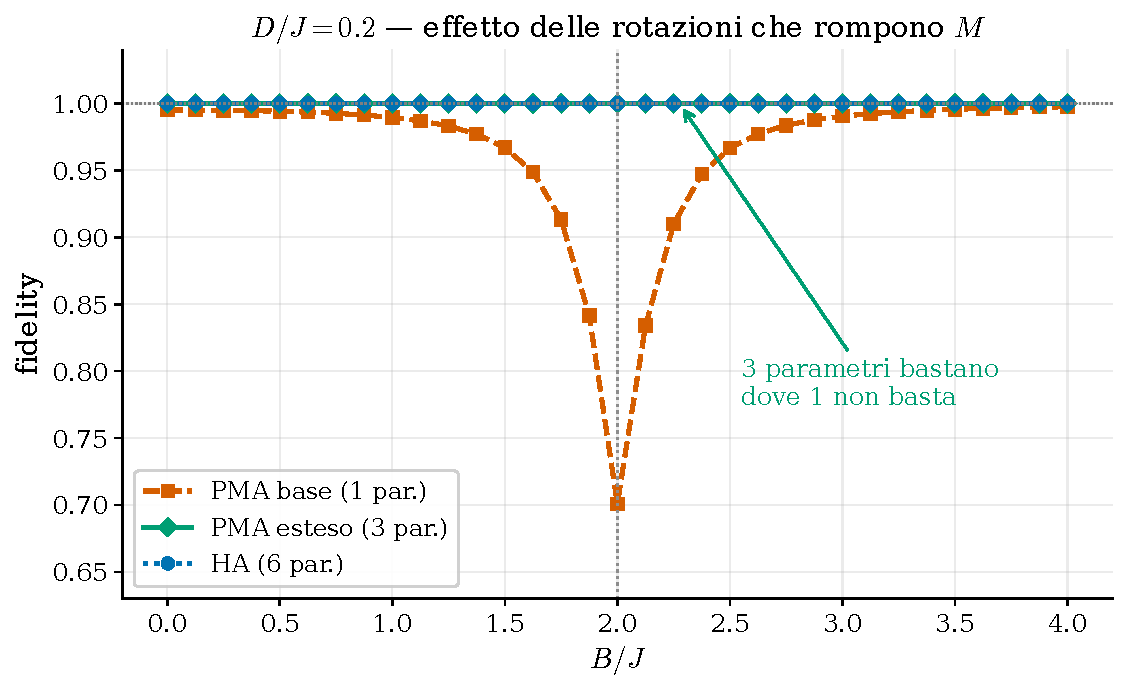
\includegraphics[width=0.78\textwidth]{figure/fig04_vqe_riparazione}
\caption{Con il DM acceso: l'ansatz a tre parametri raggiunge la fidelity
massima su tutto il range, esattamente come quello generico a sei. Metà dei
parametri, stesso risultato --- e a differenza dell'ansatz generico, ogni
parametro corrisponde a un'operazione di cui si sa dire il ruolo fisico.}
\label{fig:riparazione}
\end{figure}

\FloatBarrier

\verifica{Tutti i punti delle figure provengono da ottimizzazioni indipendenti
con $8$ punti di partenza casuali ciascuna, per escludere che una curva bassa
sia un minimo locale invece di un limite strutturale. La fidelity è calcolata
come proiezione sul \emph{sottospazio} fondamentale, non su un singolo
autovettore:
\begin{equation*}
\mathcal F = \sqrt{\textstyle\sum_{k:\,E_k\approx E_0} \lvert\langle v_k|\psi_{\rm ansatz}\rangle\rvert^2},
\end{equation*}
dove la somma corre su \emph{tutti} gli autovettori $v_k$ degeneri col
fondamentale, non su uno solo: a $D=0$ e $B/J=2$ lo stato fondamentale è
degenere, e confrontarsi con un autovettore arbitrario restituito dalla
diagonalizzazione darebbe un numero privo di significato. Al punto di lavoro
``test 2'' ($b/J=0.35$, $D/J=0.80$) l'ansatz esteso dà un errore in energia di
$4\times10^{-13}$ e $\mathcal F=1.000000000000$.}

\section{Che cosa si porta via da qui}

Il risultato utilizzabile non è ``il VQE funziona sul dimero'' --- lo si sapeva.
È il criterio di progetto: \textbf{un ansatz va costruito sulle simmetrie che
l'Hamiltoniana ha davvero, non su quelle che sarebbe comodo avesse.} Questo
criterio è stato poi applicato tale e quale a $N=3$, dove la verifica diretta è
più costosa e conviene sapere in anticipo cosa cercare.

Resta un punto aperto, questa volta non sulla scelta del gate (chiarita in
Sez.~\ref{sec:rbs-vs-w}) ma sulla sua collocazione: se e come estendere questo
stesso confronto RBS/$W$ quando l'ansatz verrà applicato a $N=3$, dove il
sottospazio a magnetizzazione fissata è più grande e la scelta del blocco
potrebbe pesare di più sul conteggio totale dei gate.

\subsection*{Un'anticipazione: lo stesso confronto, al punto del Documento 3}

Il Documento 3 sceglie un punto di lavoro diverso da quelli usati fin qui ---
$b/J=-0.18$, $D/J=1$, con un termine DM cinque volte più forte del $D/J=0.2$
di Fig.~\ref{fig:confronto} --- per ragioni che riguardano la dinamica
temporale, non l'ottimizzazione. Vale la pena controllare se il confronto fra
i tre ansatz di questo documento regge anche in quel punto, prima di darlo per
scontato:

\begin{table}[htbp]
\centering
\small
\renewcommand{\arraystretch}{1.3}
\begin{tabular}{@{}llc@{}}
\toprule
\rowcolor{grigetto}
\textbf{ansatz (nome nel testo)} & \textbf{etichetta nelle figure} & \textbf{fidelity a $b/J=-0.18$, $D/J=1$} \\
\midrule
generico, hardware-efficient (Fig.~\ref{fig:confronto}) & HA (6 par.) & $1.000000$ \\
fisicamente motivato, minimo (Fig.~\ref{fig:confronto}) & PMA base (1 par.) & $0.922857$ \\
fisicamente motivato, esteso (Fig.~\ref{fig:riparazione}) & PMA esteso (3 par.) & $1.000000$ \\
\bottomrule
\end{tabular}
\caption{Lo stesso confronto delle Fig.~\ref{fig:confronto}
e~\ref{fig:riparazione}, ricalcolato al punto di lavoro che userà il
Documento 3. Anche con un DM cinque volte più forte la storia non cambia:
l'ansatz base perde una fetta di fidelity non trascurabile, quello esteso
resta indistinguibile dall'esatto ($\mathcal F=1$ a dodici cifre). Questi
numeri tornano nel Documento 3, dove ne segue direttamente la dinamica
temporale.}
\label{tab:preview-doc3}
\end{table}

\FloatBarrier

\bigskip
\noindent\footnotesize\textit{Riferimento.} Per le rotazioni di Givens
(l'origine del nome, e il loro uso classico nell'algebra lineare
numerica): W.~Givens, \emph{Computation of Plane Unitary Rotations
Transforming a General Matrix to Triangular Form}, J.~Soc.\ Indust.\ Appl.\
Math.\ \textbf{6}(1), 26--50 (1958); trattazione moderna in G.~H.~Golub,
C.~F.~Van Loan, \emph{Matrix Computations}, Johns Hopkins University Press,
4ª ed.\ (2013), \S5.1.

\noindent\textit{Riferimento.} Per la famiglia iSWAP (il gate e la sua
origine dall'interazione $XY$ fra due qubit): N.~Schuch, J.~Siewert,
\emph{Natural two-qubit gate for quantum computation using the $XY$
interaction}, Phys.\ Rev.\ A \textbf{67}, 032301 (2003).

\noindent\textit{Riferimento.} Per la fidelity, inclusa la sua estensione
naturale a un sottospazio degenere (proiettare invece di confrontare con un
singolo vettore): M.~A.~Nielsen, I.~L.~Chuang, \emph{Quantum Computation and
Quantum Information}, Cambridge University Press, ediz.\ del decimo
anniversario (2010), cap.~9.

\end{document}
